\section{Level 1.3: Historically Structured Open Discovery}
\label{sec:level13}

\subsection{Experimental design}
\label{sec:level13-design}

Level 1.3's own Stage 0 preregistration manifest freezes the historical
mechanisms' activation ranges, the pooled discovery design, and a
mandatory mechanism-substream random-number-generator mode for every
causal run, before any Stage 1 or later run executed. Nine stages
followed: mechanism-activation calibration and a small open pilot
(Stages 1--2); a 72-run matched-seed sequencing/ordering factorial over
six pressure-onset orderings, holding cumulative exposure matched (Stage
3); a 96-run open pressure-history search (Stage 4); a 48-run (16 seeds
$\times$ 3 arms: base, erased, reversed) matched-seed causal counterfactual
on the security-pressure channel (Stage 5); a blind discovery run pooling
Stages 3--5's 216 seed-run phenotype vectors (Stage 6); a 12-run fresh,
disjoint confirmation pool (Stage 7); an $S_{\text{obs}}$--$Z_{\text{obs}}$
coupling analysis pooling all 228 available runs (Stage 8); and a
24-run scale-robustness check (Stage 9). A genuine, disclosed bug (a
two-layer activation-flag defect, this project's own task \#109) was found
and fixed in the pressure-transmission wiring during Stage 1 calibration,
before any Stage 3+ result was collected.

\subsection{Ordering and counterfactual evidence for a real historical effect}
\label{sec:level13-ordering}

Stage 3's 72-run matched factorial, holding each ordering's cumulative
pressure exposure matched, found a real, if modest, ordering-dependent
spread in $S_{\text{obs}}$/$Z_{\text{obs}}$ across the six tested onset
orderings (approximately 6--7.5\% relative spread), descriptive rather
than resampling-based at this milestone (\cref{fig:l13-ordering}). Stage
5's 16 matched seed-triples (base, erased, reversed pressure history,
single security-pressure channel by disclosed design) found a real,
directionally consistent divergence: mean $|S_{\text{obs}}|$ difference
erased-versus-base $\approx0.0027$, reversed-versus-base $\approx0.0116$,
with 1 of 16 and 3 of 16 seeds respectively showing a qualitative shift in
the sequencing vector itself (\cref{fig:l13-counterfactual}). Neither
result was independently resampled with a bootstrap confidence interval at
this milestone --- Level 1.3b's own purpose-designed Stage 3/6
(\cref{sec:level13b}) is the direct confirmatory successor to both.

\subsection{Discovery result and fresh-data reproduction failure}
\label{sec:level13-discovery}

Stage 6's blind discovery run, pooling Stages 3--5's 216 seed-run phenotype
vectors, reached headline $k=2$ with silhouette 0.334 (silhouette by $k$:
0.334, 0.256, 0.285, 0.297, 0.153, 0.196, 0.297 for $k=2$ through 8) and a
bootstrap stability mean adjusted Rand index of 0.917 (30 resamples) ---
a genuinely stable in-sample fit. Two pieces of evidence, however, argue
directly against reading this as a discrete two-family finding. First,
cross-algorithm agreement was only modest (mean adjusted Rand index
$\approx0.291$), and \texttt{HDBSCAN} found zero clusters on this feature
space entirely. Second, and decisively, Stage 7's disjoint 12-run fresh
confirmation pool --- scoring Stage 6's own frozen fit on data it never
saw --- failed to reproduce it: per-run log-likelihood degraded from
$\approx-1.29$ on the training pool to $\approx-6.05$ on the fresh pool, a
sharp collapse, and every one of the 12 fresh points fell into a single
cluster. A further disclosed confound, $\text{cluster\_vs\_source\_stage}$
adjusted Rand index $\approx0.554$, shows the pooled 216-point discovery
sample is not ecologically homogeneous (cluster assignment partially
tracks which of Stages 3/4/5 a point came from), a genuine limitation of a
pooled, not purpose-designed, discovery sample that Level 1.3b's own Stage
4 (\cref{sec:level13b}) was built specifically to avoid.

Applying Level 1.2b's own frozen \texttt{classify\_discovery\_verdict}
function unmodified to this evidence, Level 1.3's formal six-way
classification is \texttt{D\_continuum}, with \texttt{B\_two\_families}
identified explicitly as the closest runner-up rather than a rejected
alternative --- the same evidentiary caution this paper's own
terminological discipline (\cref{sec:terminology-discipline}) requires.

\subsection{\texorpdfstring{The $S_{\text{obs}}$--$Z_{\text{obs}}$ coupling}{The S\_obs--Z\_obs coupling}}
\label{sec:level13-coupling}

Pooling all 228 runs available across Stages 3, 4, 5, and 7, the observer-
side $S_{\text{obs}}$--$Z_{\text{obs}}$ correlation is strong: Pearson
$r=0.888$ ($p\approx2.4\times10^{-78}$), Spearman $\rho=0.913$
($p\approx3.8\times10^{-90}$), $n=228$ (\cref{fig:l13-coupling}). This is
descriptive and correlational, not yet audited at this milestone for
whether the coupling reflects genuine construct independence, a
shared-construction artifact, or a common behavioral driver --- an open
question Level 1.3 itself explicitly leaves for the next milestone. Stage
9's own coarser check (24 runs across four scale cells) found
$S_{\text{obs}}$ and $Z_{\text{obs}}$ ``qualitatively stable''
($S_{\text{obs}}\in[0.649,0.710]$, $Z_{\text{obs}}\in[0.438,0.470]$), a
suggestive but not dispositive check reported as such rather than as a
formal stability statistic.

\subsection{Why a purpose-designed successor was still required}
\label{sec:level13-why-1.3b}

Level 1.3's own record, audited claim by claim in a dedicated inference
audit before Level 1.3b's own preregistration was frozen, was found free
of fabrication or miscitation, but resting almost entirely on one pooled,
216-to-228-run sample assembled after the fact from Stages 3--5, with only
one genuinely independent fresh-data test (Stage 7's 12 points) --- exactly
the one claim that failed to reproduce. \Cref{sec:level13b} reports the
purpose-designed, preregistered, causally instrumented successor this
motivates.

\begin{figure}[htbp]
\centering
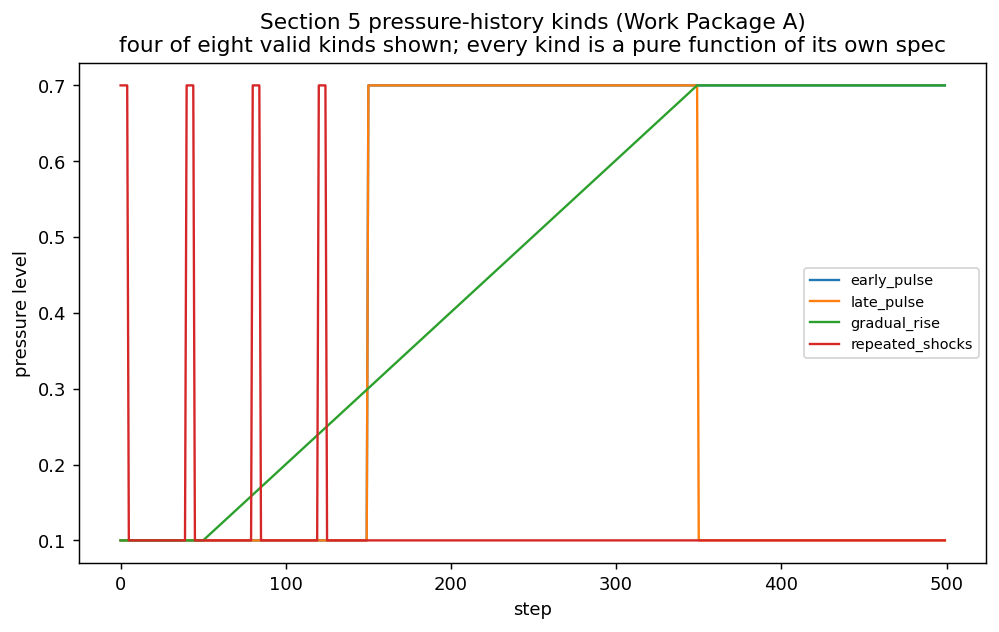
\includegraphics[width=0.85\textwidth]{figures/appendix/a_l13_pressure_history_kinds.png}
\caption{Level 1.3's three pressure channels (security, bargaining,
coordination-complexity) and the pressure-history transforms (base,
erased, reversed) used in Stage 5's matched-seed counterfactual design.}
\label{fig:l13-ordering}
\end{figure}

\begin{figure}[htbp]
\centering
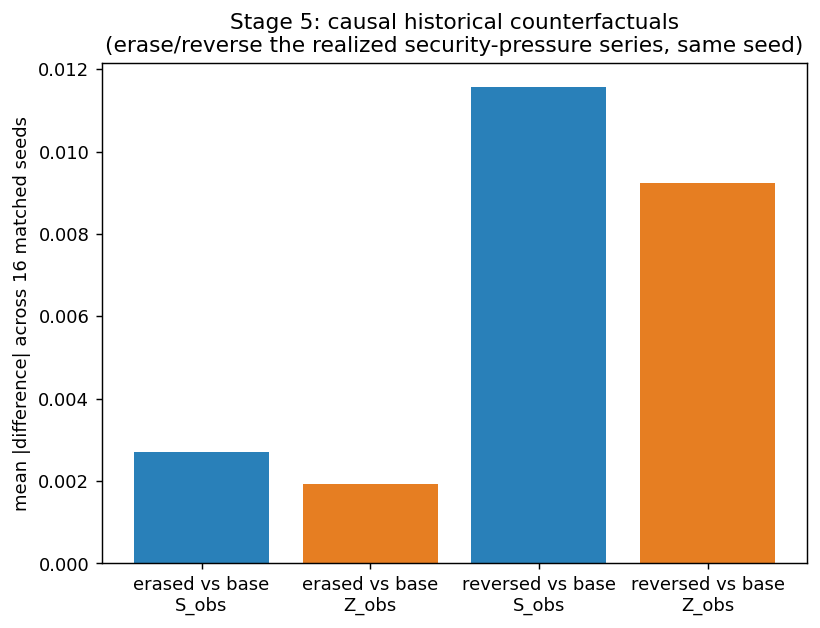
\includegraphics[width=0.85\textwidth]{figures/appendix/a_l13_counterfactual_shift.png}
\caption{Level 1.3 Stage 5: matched-seed counterfactual shift in
$S_{\text{obs}}$/$Z_{\text{obs}}$ for erased and reversed pressure history
versus the base run (16 matched triples, security-pressure channel only).
Descriptive, single-channel; not yet resampled with a bootstrap CI at this
milestone.}
\label{fig:l13-counterfactual}
\end{figure}

\begin{figure}[htbp]
\centering
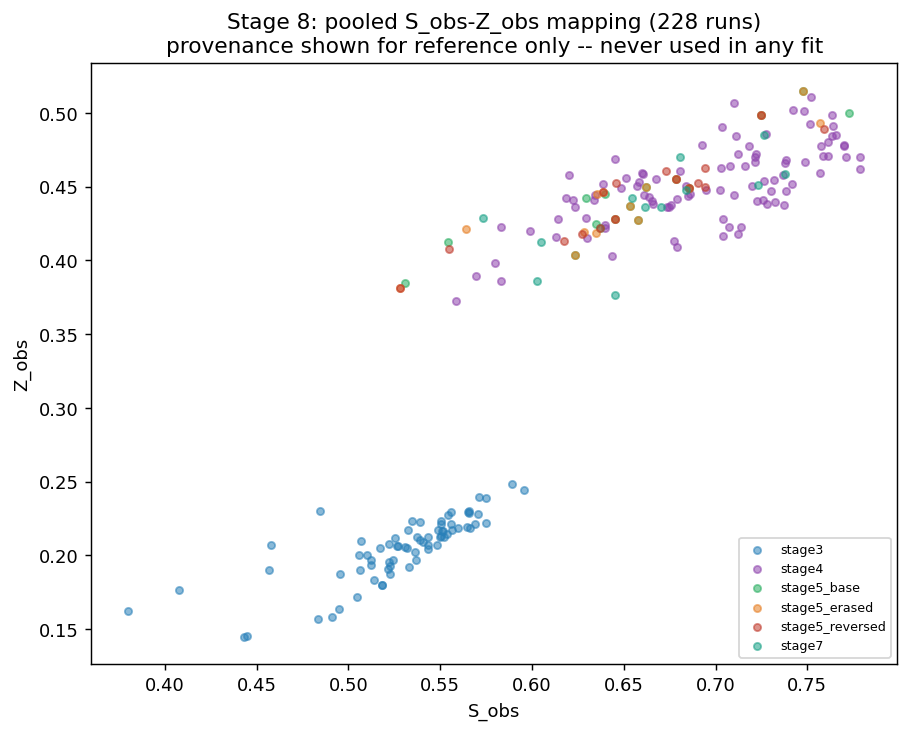
\includegraphics[width=0.85\textwidth]{figures/level13b/l13_fig1_s_obs_z_obs_scatter.png}
\caption{Level 1.3 Stage 8: $S_{\text{obs}}$ versus $Z_{\text{obs}}$ across
all 228 pooled runs (Stages 3/4/5/7). Pearson $r=0.888$, Spearman
$\rho=0.913$. Descriptive correlation; construct-independence audit
deferred to Level 1.3b Stage 9 (\cref{sec:level13b-measurement}).}
\label{fig:l13-coupling}
\end{figure}
